\documentclass[12pt,a4paper,fleqn]{article}
\usepackage[utf8]{inputenc}
\usepackage[russian]{babel}
\usepackage{amssymb, amsmath, multicol}
\usepackage{enumitem}
\usepackage{lipsum}
\usepackage{euler}
\oddsidemargin=-15.4mm
\textwidth=190mm
\headheight=-32.4mm
\textheight=277mm
\parindent=0pt
\parskip=8pt
\pagestyle{empty}
\usepackage{graphicx}
\begin{document}
\begin{center}
\textbf{\LARGE{Исследовательская работа по теме:\\Исследование функции дифференциальными методами}}\end{center}\newpage\textbf{\LARGE{Глава I. Функция}}

\begin{center}
$y = $$\frac{sin(log(x^{cos(x)}))}{log((1-(5 \cdot x^{3})))}$

\end{center}
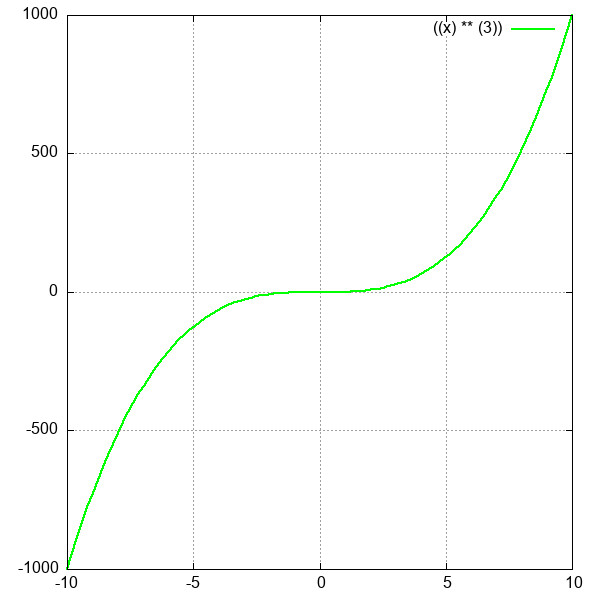
\includegraphics{GraphicDumps/plot.jpg}\newpage \textbf{\LARGE{Глава II. Визуальный анализ функции}}

Руководствуясь сборником <<Задачи для подготовки к поступлению в советские ясли>>

\begin{center}
$y = $$\frac{sin(log(x^{cos(x)}))}{log((1-(5 \cdot x^{3})))}$

\end{center}
\newpage \textbf{\LAGRE{Глава III. Дифференцирование}}

Таким образом

\begin{center}
 ($x)'
  = 1$\end{center}
Обоснование этого перехода было забанено редактурой

\begin{center}
 ($x)'
  = 1$\end{center}
Segmentation fault (core dumped)

\begin{center}
 ($cos(x))'
  = (1 \cdot (0-sin(x)))$\end{center}
Таким образом

\begin{center}
A = $((\frac{cos(x)}{x} \cdot 1)+((1 \cdot (0-sin(x))) \cdot log(x)))$\end{center}
\begin{center}
 ($x^{cos(x)})'
  = (x^{cos(x)} \cdot A)$\end{center}
Господи, да для кого я вообще стараюсь

\begin{center}
A = $((\frac{cos(x)}{x} \cdot 1)+((1 \cdot (0-sin(x))) \cdot log(x)))$\end{center}
\begin{center}
 ($log(x^{cos(x)}))'
  = (\frac{1}{x^{cos(x)}} \cdot (x^{cos(x)} \cdot A))$\end{center}
Ну ты же всё равно не будешь это проверять

\begin{center}
A = $((\frac{cos(x)}{x} \cdot 1)+((1 \cdot (0-sin(x))) \cdot log(x)))$\end{center}
\begin{center}
B = $(\frac{1}{x^{cos(x)}} \cdot (x^{cos(x)} \cdot A))$\end{center}
\begin{center}
 ($sin(log(x^{cos(x)})))'
  = (B \cdot cos(log(x^{cos(x)})))$\end{center}
Первая производная комом

\begin{center}
 ($1)'
  = 0$\end{center}
Отметим, что

\begin{center}
 ($5)'
  = 0$\end{center}
Руководствуясь сборником <<Задачи для подготовки к поступлению в советские ясли>>

\begin{center}
 ($x)'
  = 1$\end{center}
Вы не шокированы?

\begin{center}
 ($x^{3})'
  = (((3-1) \cdot x^{(3-1)}) \cdot 1)$\end{center}
ИИИИЕЕЕЕсли

\begin{center}
A = $(((3-1) \cdot x^{(3-1)}) \cdot 1)$\end{center}
\begin{center}
 ($(5 \cdot x^{3}))'
  = ((0 \cdot x^{3})+(5 \cdot A))$\end{center}
Только 0.00001 процент умнейших людей планеты смогут понять этот переход

\begin{center}
A = $(((3-1) \cdot x^{(3-1)}) \cdot 1)$\end{center}
\begin{center}
 ($(1-(5 \cdot x^{3})))'
  = (0-((0 \cdot x^{3})+(5 \cdot A)))$\end{center}
Телец в козероге, поэтому

\begin{center}
A = $(((3-1) \cdot x^{(3-1)}) \cdot 1)$\end{center}
\begin{center}
B = $(0-((0 \cdot x^{3})+(5 \cdot A)))$\end{center}
\begin{center}
 ($log((1-(5 \cdot x^{3}))))'
  = (\frac{1}{(1-(5 \cdot x^{3}))} \cdot B)$\end{center}
Используя выводы из теоремы 1000-7 получаем

\begin{center}
A = $((\frac{cos(x)}{x} \cdot 1)+((1 \cdot (0-sin(x))) \cdot log(x)))$\end{center}
\begin{center}
B = $(\frac{1}{x^{cos(x)}} \cdot (x^{cos(x)} \cdot A))$\end{center}
\begin{center}
C = $((B \cdot cos(log(x^{cos(x)}))) \cdot log((1-(5 \cdot x^{3}))))$\end{center}
\begin{center}
D = $(((3-1) \cdot x^{(3-1)}) \cdot 1)$\end{center}
\begin{center}
E = $(0-((0 \cdot x^{3})+(5 \cdot D)))$\end{center}
\begin{center}
F = $(\frac{1}{(1-(5 \cdot x^{3}))} \cdot E)$\end{center}
\begin{center}
G = $(log((1-(5 \cdot x^{3}))) \cdot log((1-(5 \cdot x^{3}))))$\end{center}
\begin{center}
 ($\frac{sin(log(x^{cos(x)}))}{log((1-(5 \cdot x^{3})))})'
  = \frac{(C-(F \cdot sin(log(x^{cos(x)}))))}{G}$\end{center}
\newpage \textbf{\LARGE{Глава IV.Упрощение выражения}}

И хотя клуб любителей таких формул двумя блоками ниже, мы продолжаем

\begin{center}
\begin{center}$(3-1) = 2$\end{center}
(null)

\begin{center}
\begin{center}$(3-1) = 2$\end{center}
Доказательство данного факта предоставлено лицом или организацией исполняющей функции иностанного агента

\begin{center}
$(\frac{cos(x)}{x} \cdot 1) = \frac{cos(x)}{x}$\end{center}
Британские учёные доказали, что для поддержания мозга в тонусе необходимо ежедневно дифференцировать. Продолжим наше приобщение к здоровому образу жизниn

\begin{center}
$(1 \cdot (0-sin(x))) = (0-sin(x))$\end{center}
//TODO: Лёша, придумай переход. У меня идеи закончились

\begin{center}
$(0 \cdot x^{3}) = 0$\end{center}
Продвинутый читатель уже заметил, что

\begin{center}
$((2 \cdot x^{2}) \cdot 1) = (2 \cdot x^{2})$\end{center}
Таким образом

\begin{center}
$(0+(5 \cdot (2 \cdot x^{2}))) = (5 \cdot (2 \cdot x^{2}))$\end{center}
\newpage \textbf{\LARGE{Глава V. Полученая производная}}

$y = $$\frac{sin(log(x^{cos(x)}))}{log((1-(5 \cdot x^{3})))}$

\begin{center}
A = $(\frac{cos(x)}{x}+((0-sin(x)) \cdot log(x)))$\end{center}
\begin{center}
B = $(\frac{1}{x^{cos(x)}} \cdot (x^{cos(x)} \cdot A))$\end{center}
\begin{center}
C = $((B \cdot cos(log(x^{cos(x)}))) \cdot log((1-(5 \cdot x^{3}))))$\end{center}
\begin{center}
D = $(\frac{1}{(1-(5 \cdot x^{3}))} \cdot (0-(5 \cdot (2 \cdot x^{2}))))$\end{center}
\begin{center}
E = $(log((1-(5 \cdot x^{3}))) \cdot log((1-(5 \cdot x^{3}))))$\end{center}
$y' = $$\frac{(C-(D \cdot sin(log(x^{cos(x)}))))}{E}$

\includegraphics{GraphicDumps/plot_1.jpg}
\end{document}